\section{Introduction}

I have yet to see any problem, however complicated, which, when looked at in the right way did not become still more complicated.

\begin{flushright}--- Poul Anderson\end{flushright}

  People working in the field of high energy physics have a tendency to concern themselves with attempting to solve problems that are incredibly complicated.
  So, perhaps, there is a touch of irony that the problem that they are trying to solve is not only incredibly fundamental, but also very simple to state.
  The question can be boiled down to -- what is the stuff in our universe made of?
  What immediately follows from this fundamental inquiry is how is matter made up of these things ; or to put it another way, how do the fundamental building blocks interact.

  In some sense particle physics tries to distill matter and the interactions therein down to the smallest possible level to which it can be broken down.
  Turns out that breaking these concepts down to this elementary level of specificity is an incredibly complicated process of which we have merely begun to scratch the surface.
  As such,this paper focuses on a tiny fraction of these fundamental building blocks -- the elusive neutrino with the hope of just perhaps being able to untangle some of the myriad of secrets that it harbours.

  \subsection{The Standard Model}

  Before the protagonis
  \footnote{Really the ensemble cast, given that they come in three flavors, electron($e\nu$), muon ($\mu \nu$) and tau($\tau \nu$)and their respective antiparticles,}
  of our story - the neutrino - can be formally introduced, the stage has to be set.
  A good candidate to set the stage would be the standard model which describesthree of the four known fundamental forces, electromagnetic, weak and strong interactions (it struggles to deal with  gravity) and classifying all known elementary particles.
  Just like any foundational theory that undergirds a subfield of a subject, the standard model definitely wasn't developed in a day and as such, it may behoove us to at least go over the high points ofits development in order to have a vetter understanding of the context that surrounds neutrinos. 






  %% Heading 1 is the style you should use for the following headings in your thesis: List of Tables,
  List of Figures (List of Abbreviations, Schemes, and so on), Chapter titles, References, and Appendix titles. If you are writing in APA style, note that the titles formatted as Heading 1 do not count as an APA heading. %

  %% I want to cite something here \parencite{zuo2019standing}. I want to want to try cite~\textcite{zuo2019standing} with in-line style.

  %% \subsection{heading 2: Use for Your broadest Subheading Level, Centered, Bold, Title Case}

  %% Heading 2 is the first major subheading style. If you are writing in APA style, this heading corresponds to a Level 1 APA heading.  

  %% \subsubsection{heading 3: Use for Your Next Heading Level, Left-aligned, Bold, Title Case}

  %% Heading 3 is the second major subheading style. If you are writing in APA style, this heading corresponds to a Level 2 APA heading. 

  %% \paragraph{Heading 4: This Heading is Left-aligned, Boldface Italics, Title Case}
  %% %% This is an additional heading level, should your thesis require this level of specificity.

  %% %% Let me add a figure here~\cref{fig:1}:
  %% %% \begin{figure}[h]
  %% %%     \centering
  %% %%     \captionsetup{width=0.6\linewidth} %% change width to adjust the caption alignment
  %%     \caption{Old capital museum} %
  %%     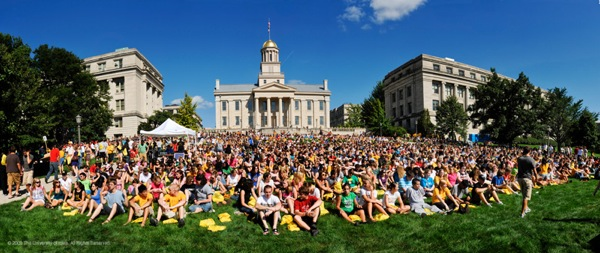
\includegraphics[width=0.6\columnwidth]{fig1}
  %%     \label{fig:1}
  %% \end{figure}                    %
  %% %% 
